
	El algoritmo de Kalman se basa en poder estimar el vector de estados a partir de la dinámica del sistema y las mediciones. Para la definición del algoritmo se utilizará la siguiente notación. Se llamará:
	
	\begin{equation*}
		\vect{x_{k/k - 1}}
	\end{equation*}
	a la mejor estimación del vector de estados utilizando información hasta el instante $k - 1$. Es decir se trata de una predicción. Se llamará a la matriz de covarianza del error de dicha estimacion:
	
	\begin{equation*}
		\vect{P_{k/k - 1}}
	\end{equation*}
	
	Por otro lado se llamará a:
	
	\begin{equation*}
		\vect{x_{k/k}}
	\end{equation*}
	a la mejor estimación del vector de estados utilizando información hasta el instante $k$. Dicha estimación será el resultado final del algoritmo y la matriz de covarianza del error del mismo será:
	
	\begin{equation*}
		\vect{P_{k/k - 1}}
	\end{equation*}

	Cabe aclarar que cuando se habla del mejor estimador, se referiere a aquel que minimiza el error cuadrático medio.\\
	
		\subsection{Algoritmo de Kalman}
			\paragraph{Inicialización}
				Es la etapa en la cual se define el estado inicial de la estimación. Para poder inicializar el algoritmo se necesita una estadistica del estado inicial del sistema:
				
				\begin{equation*}
					\vect{x_{0/0}} \leftarrow E\left[\vect{x_{0}}\right]
				\end{equation*}
				
				\begin{equation*}
					P_{0/0} \leftarrow \text{cov}\left[\vect{x_{0}}\right]
				\end{equation*}
			\paragraph{Predicción}
				Es la etapa en la cual se realiza una predicción del futuro estado del sistema utilizando el modelo en el espacio de estados:
				
				\begin{equation*}
					\vect{x_{k/k - 1}} \leftarrow Ad_{k - 1} \vect{x_{k - 1/k - 1}}
				\end{equation*}
				
				\begin{equation*}
					P_{k/k - 1} \leftarrow Ad_{k - 1} P_{k - 1 / k - 1} Ad_{k - 1}^{*} + Bd_{k - 1} Q_{k - 1} Bd_{k - 1}^{*}
				\end{equation*}
			\paragraph{Corrección}
				Es la etapa en la cual se corrige la predicción con el valor de la medición. Para ello se necesita calcular la matriz de ganancia de Kalman $K_{k}$:
				
				\begin{equation*}
					K_{k} \leftarrow P_{k / k - 1} Cd_{k}^{*} (Cd_{k} P_{k/k - 1} Cd_{k}^{*} + R_{k})^{-1}
				\end{equation*}
				
				Luego se corrige:
				
				\begin{equation*}
					\vect{x_{k/k}} \leftarrow \vect{x_{k/k - 1}} + K_{k} (y_{k} - Cd_{k} \vect{x_{k/k - 1}})
				\end{equation*}
				
				\begin{equation*}
					P_{k/k} \leftarrow (I - K_{k} Cd_{k}) P_{k/k - 1}
				\end{equation*}
					
			\paragraph{Actualización}
				Es la etapa del algoritmo en la que se pasa al siguiente instante $k$.
				
				\begin{equation*}
					\vect{x_{k - 1/k - 1}} \leftarrow \vect{x_{k/k}}
				\end{equation*}
				
				\begin{equation*}
					P_{k - 1/k - 1} \leftarrow P_{k/k}
				\end{equation*}


	\subsection{Resultados}
		\subsubsection{Medición De Posición}
			En la figura \ref{fig:ej2a} se observan los resultados de la estimación basada en mediciones de posición. Puede verse que la estimación se desvía menos del valor real que las mediciones.

		\begin{figure}[H]
			\centering
			%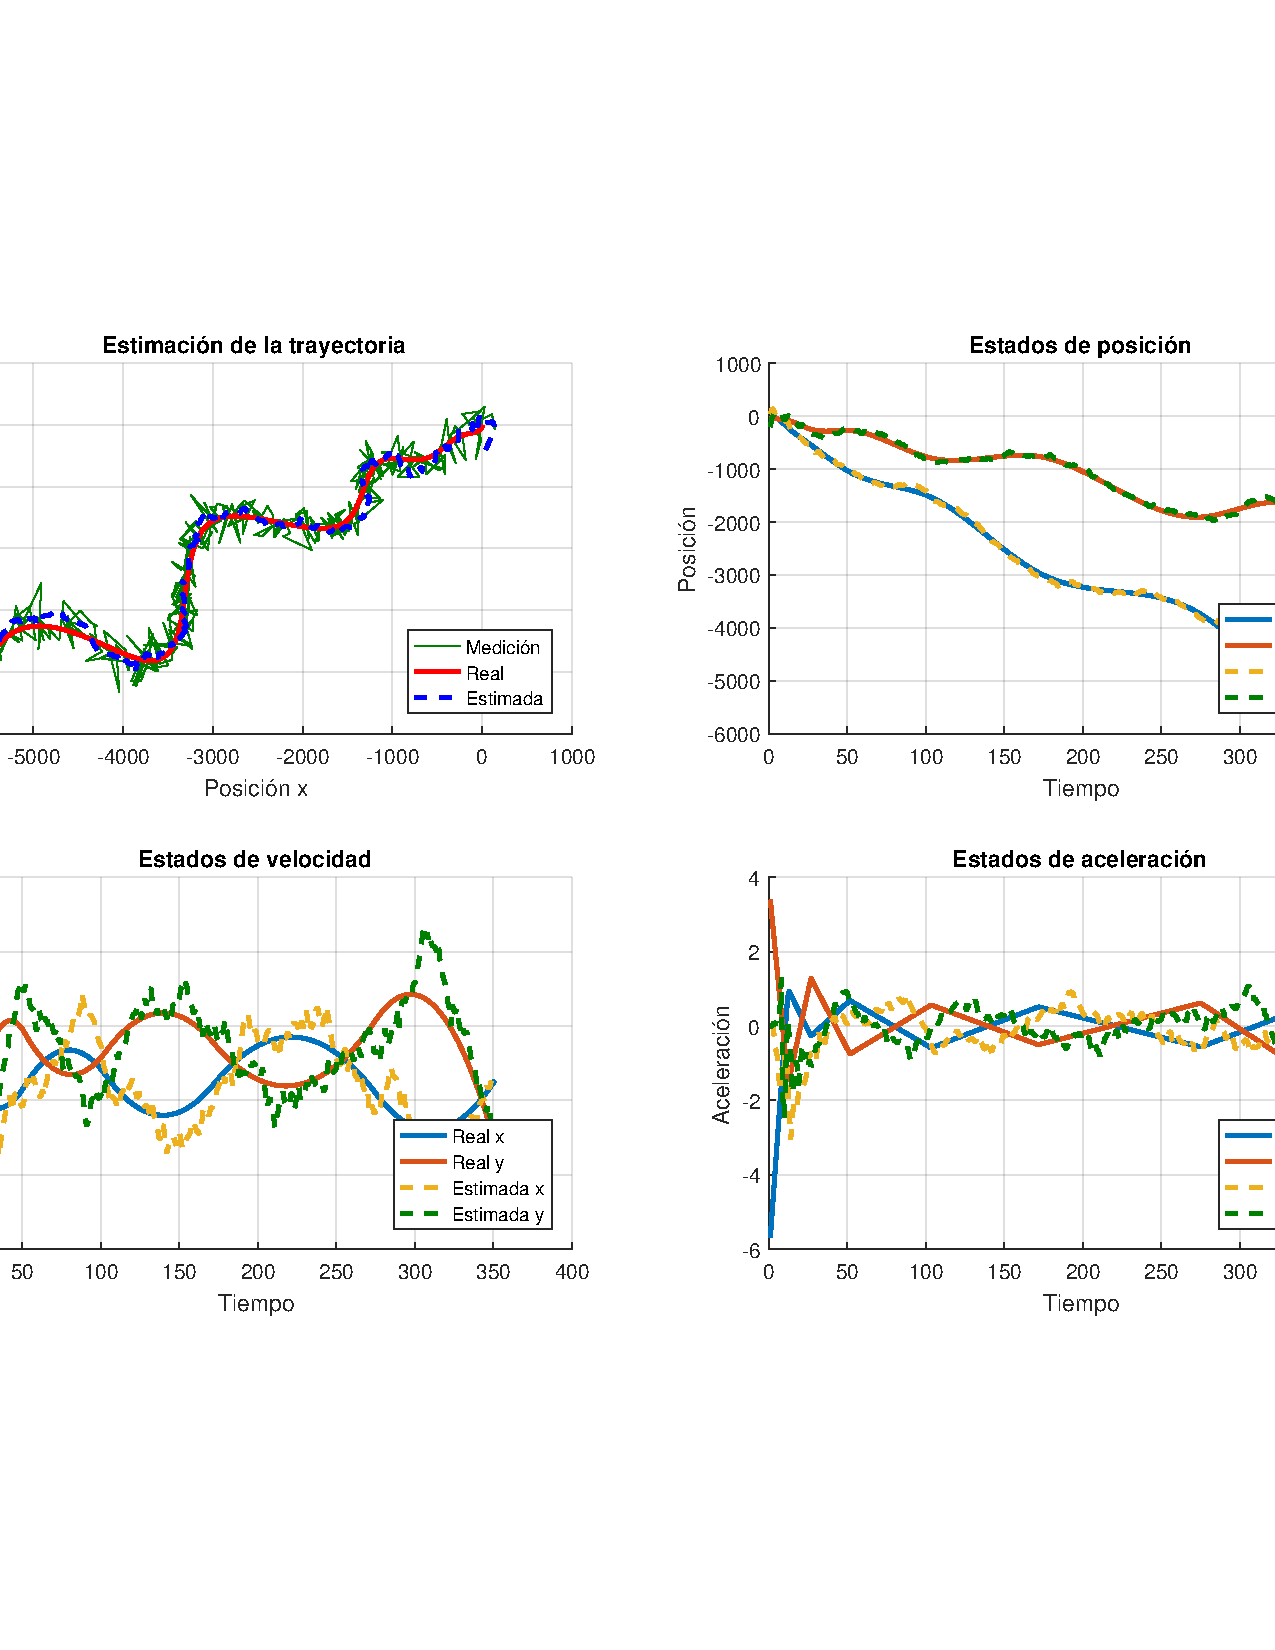
\includegraphics[width=1.0\textwidth,keepaspectratio]{Figuras/graf_ej2a.pdf}
			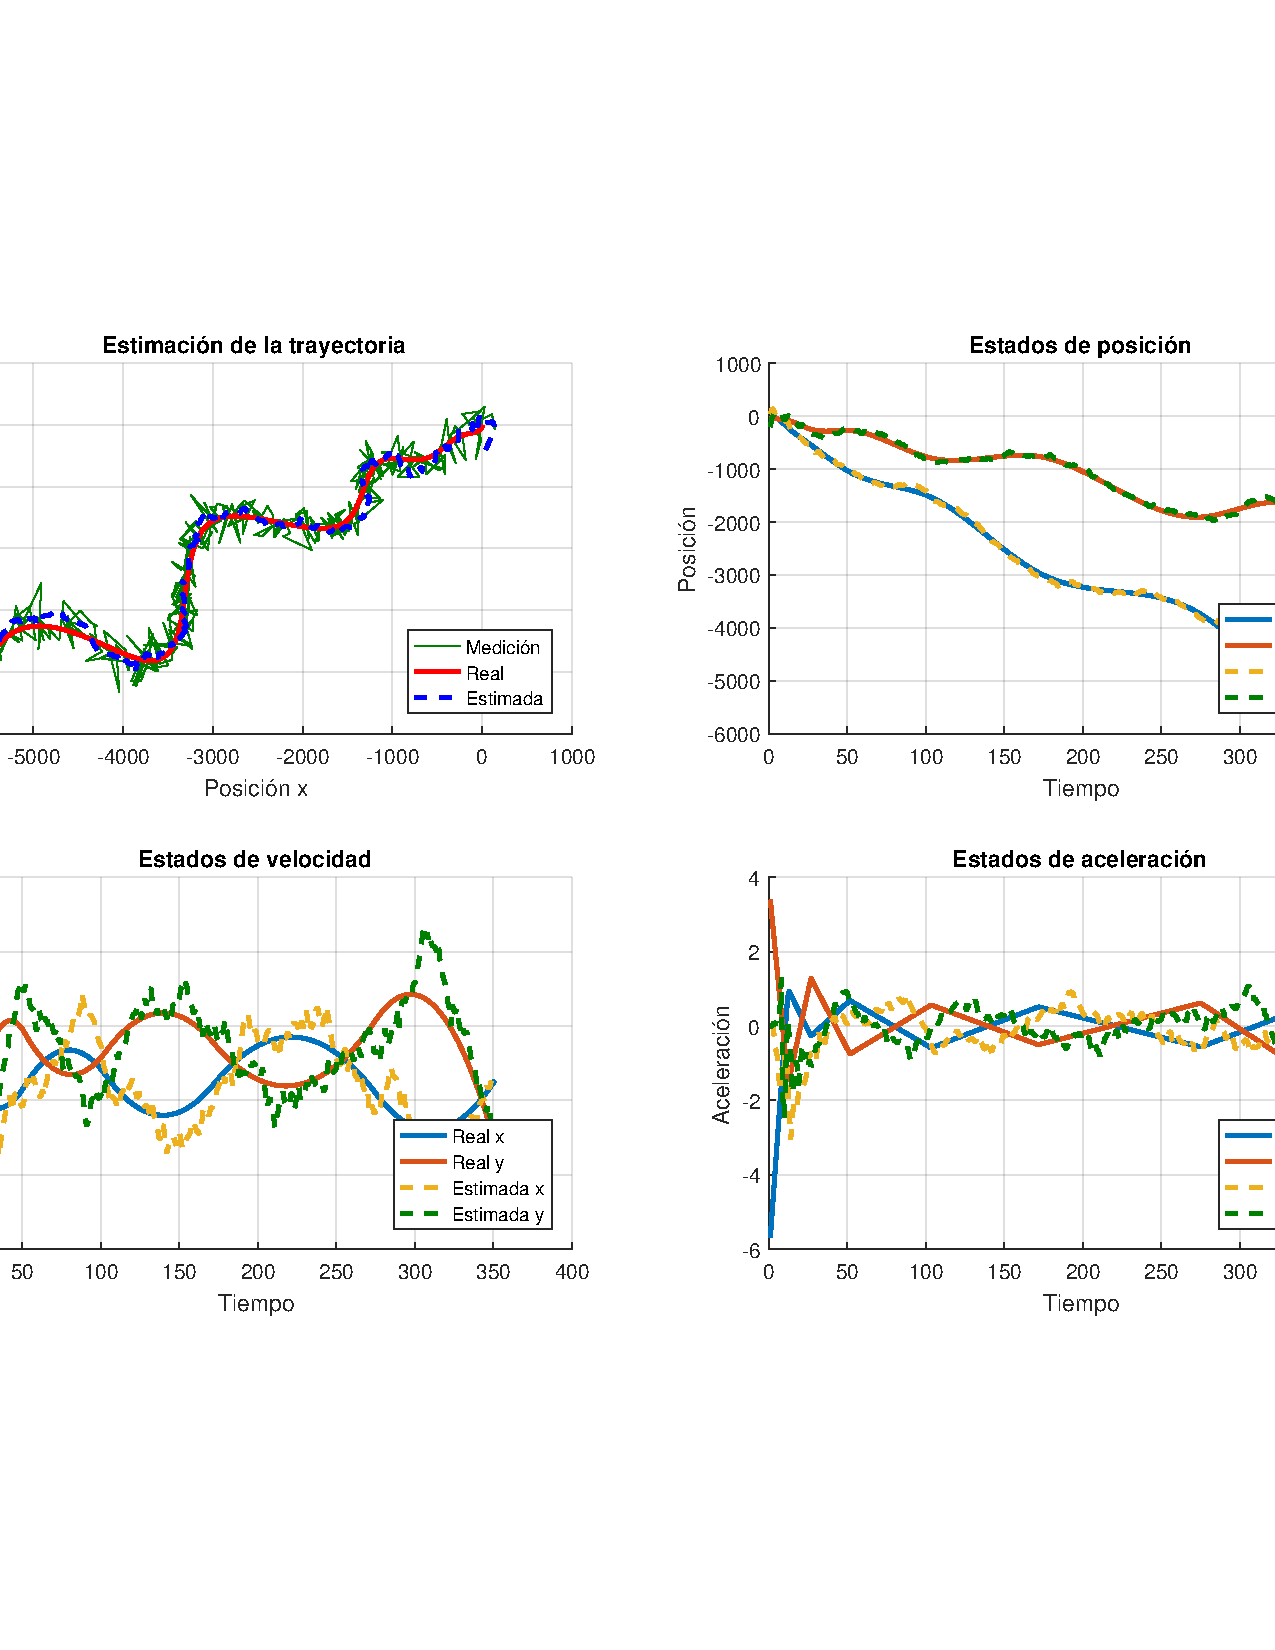
\includegraphics[scale=0.5,trim={6,5cm 0 0 0}]{Figuras/graf_ej2a.pdf}
			\caption{Caso: Medición De Posición}
			\label{fig:ej2a}
		\end{figure}
		
		En la figura \ref{fig:ej2a_innov} vemos la correlación de las innovaciones, donde se observa que se aproximan a un proceso blanco.
		
		\begin{figure}[H]
			\centering
			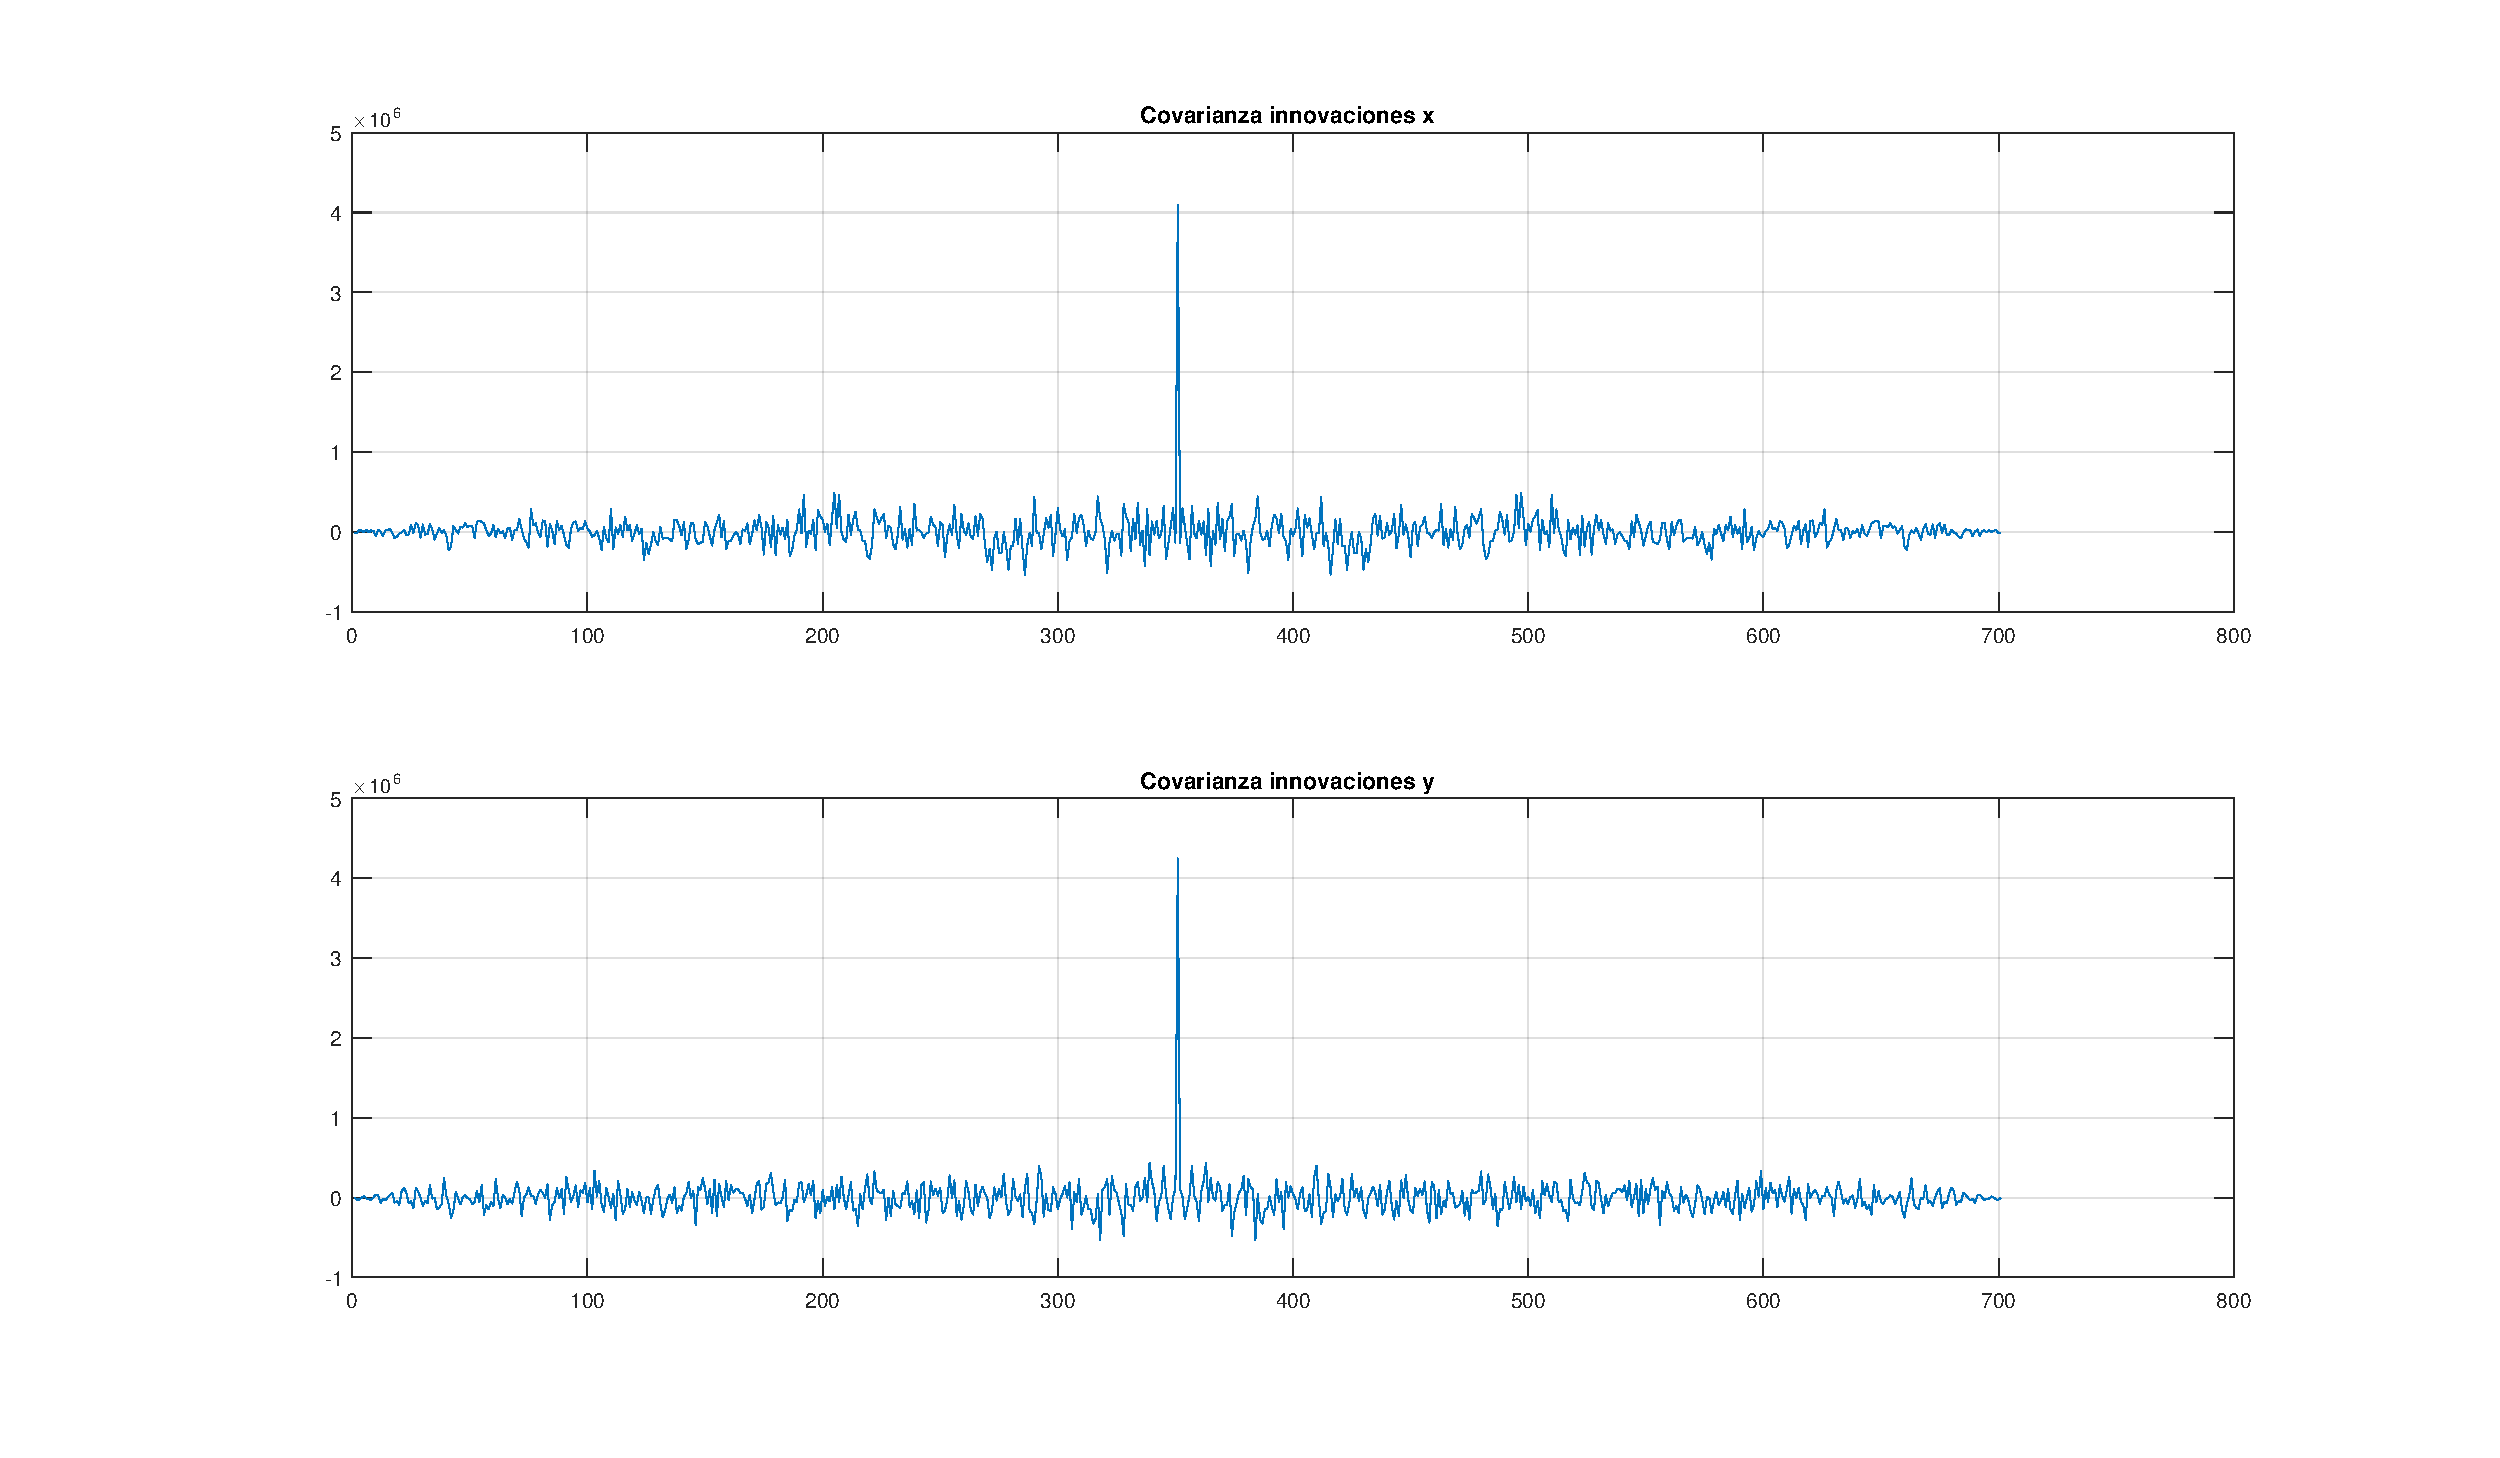
\includegraphics[width=1.0\textwidth,keepaspectratio]{Figuras/covinn_ej2a.pdf}
			\caption{Caso: Medición De Posición - Innovaciones}
			\label{fig:ej2a_innov}
		\end{figure}
		
		\subsubsection{Medición De Velocidad}
		
		En la figura \ref{fig:ej2b} observamos los resultados de la estimación basada en mediciones de velocidad. Puede verse que hay una desviación de la estimación respecto de la trayectoria real.
		
		\begin{figure}[H]
			\centering
			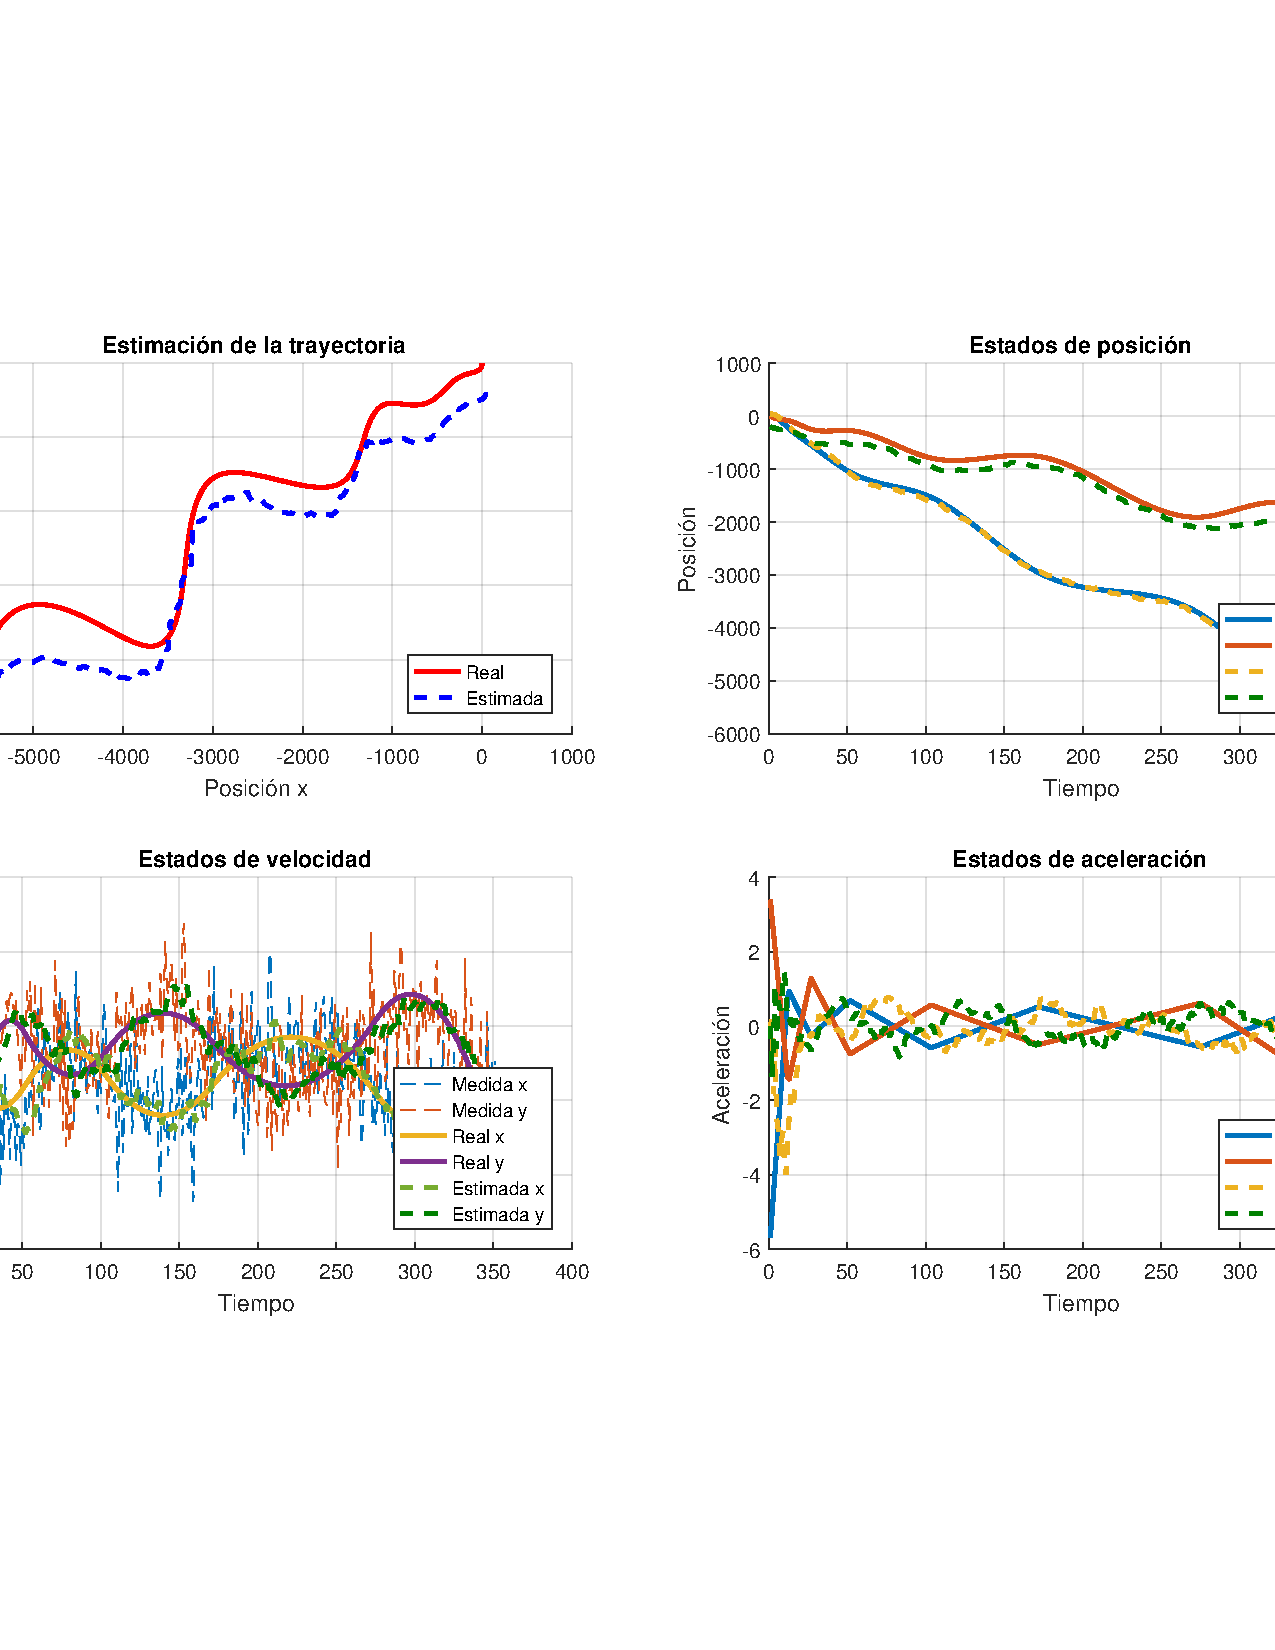
\includegraphics[scale=0.5,trim={6,5cm 0 0 0}]{Figuras/graf_ej2b.pdf}
			\caption{Caso: Medición De Velocidad}
			\label{fig:ej2b}
		\end{figure}
		
		En la figura \ref{fig:ej2b_innov} vemos la correlación de las innovaciones, donde se observa que se aproximan a un proceso blanco.
		
		\begin{figure}[H]
			\centering
			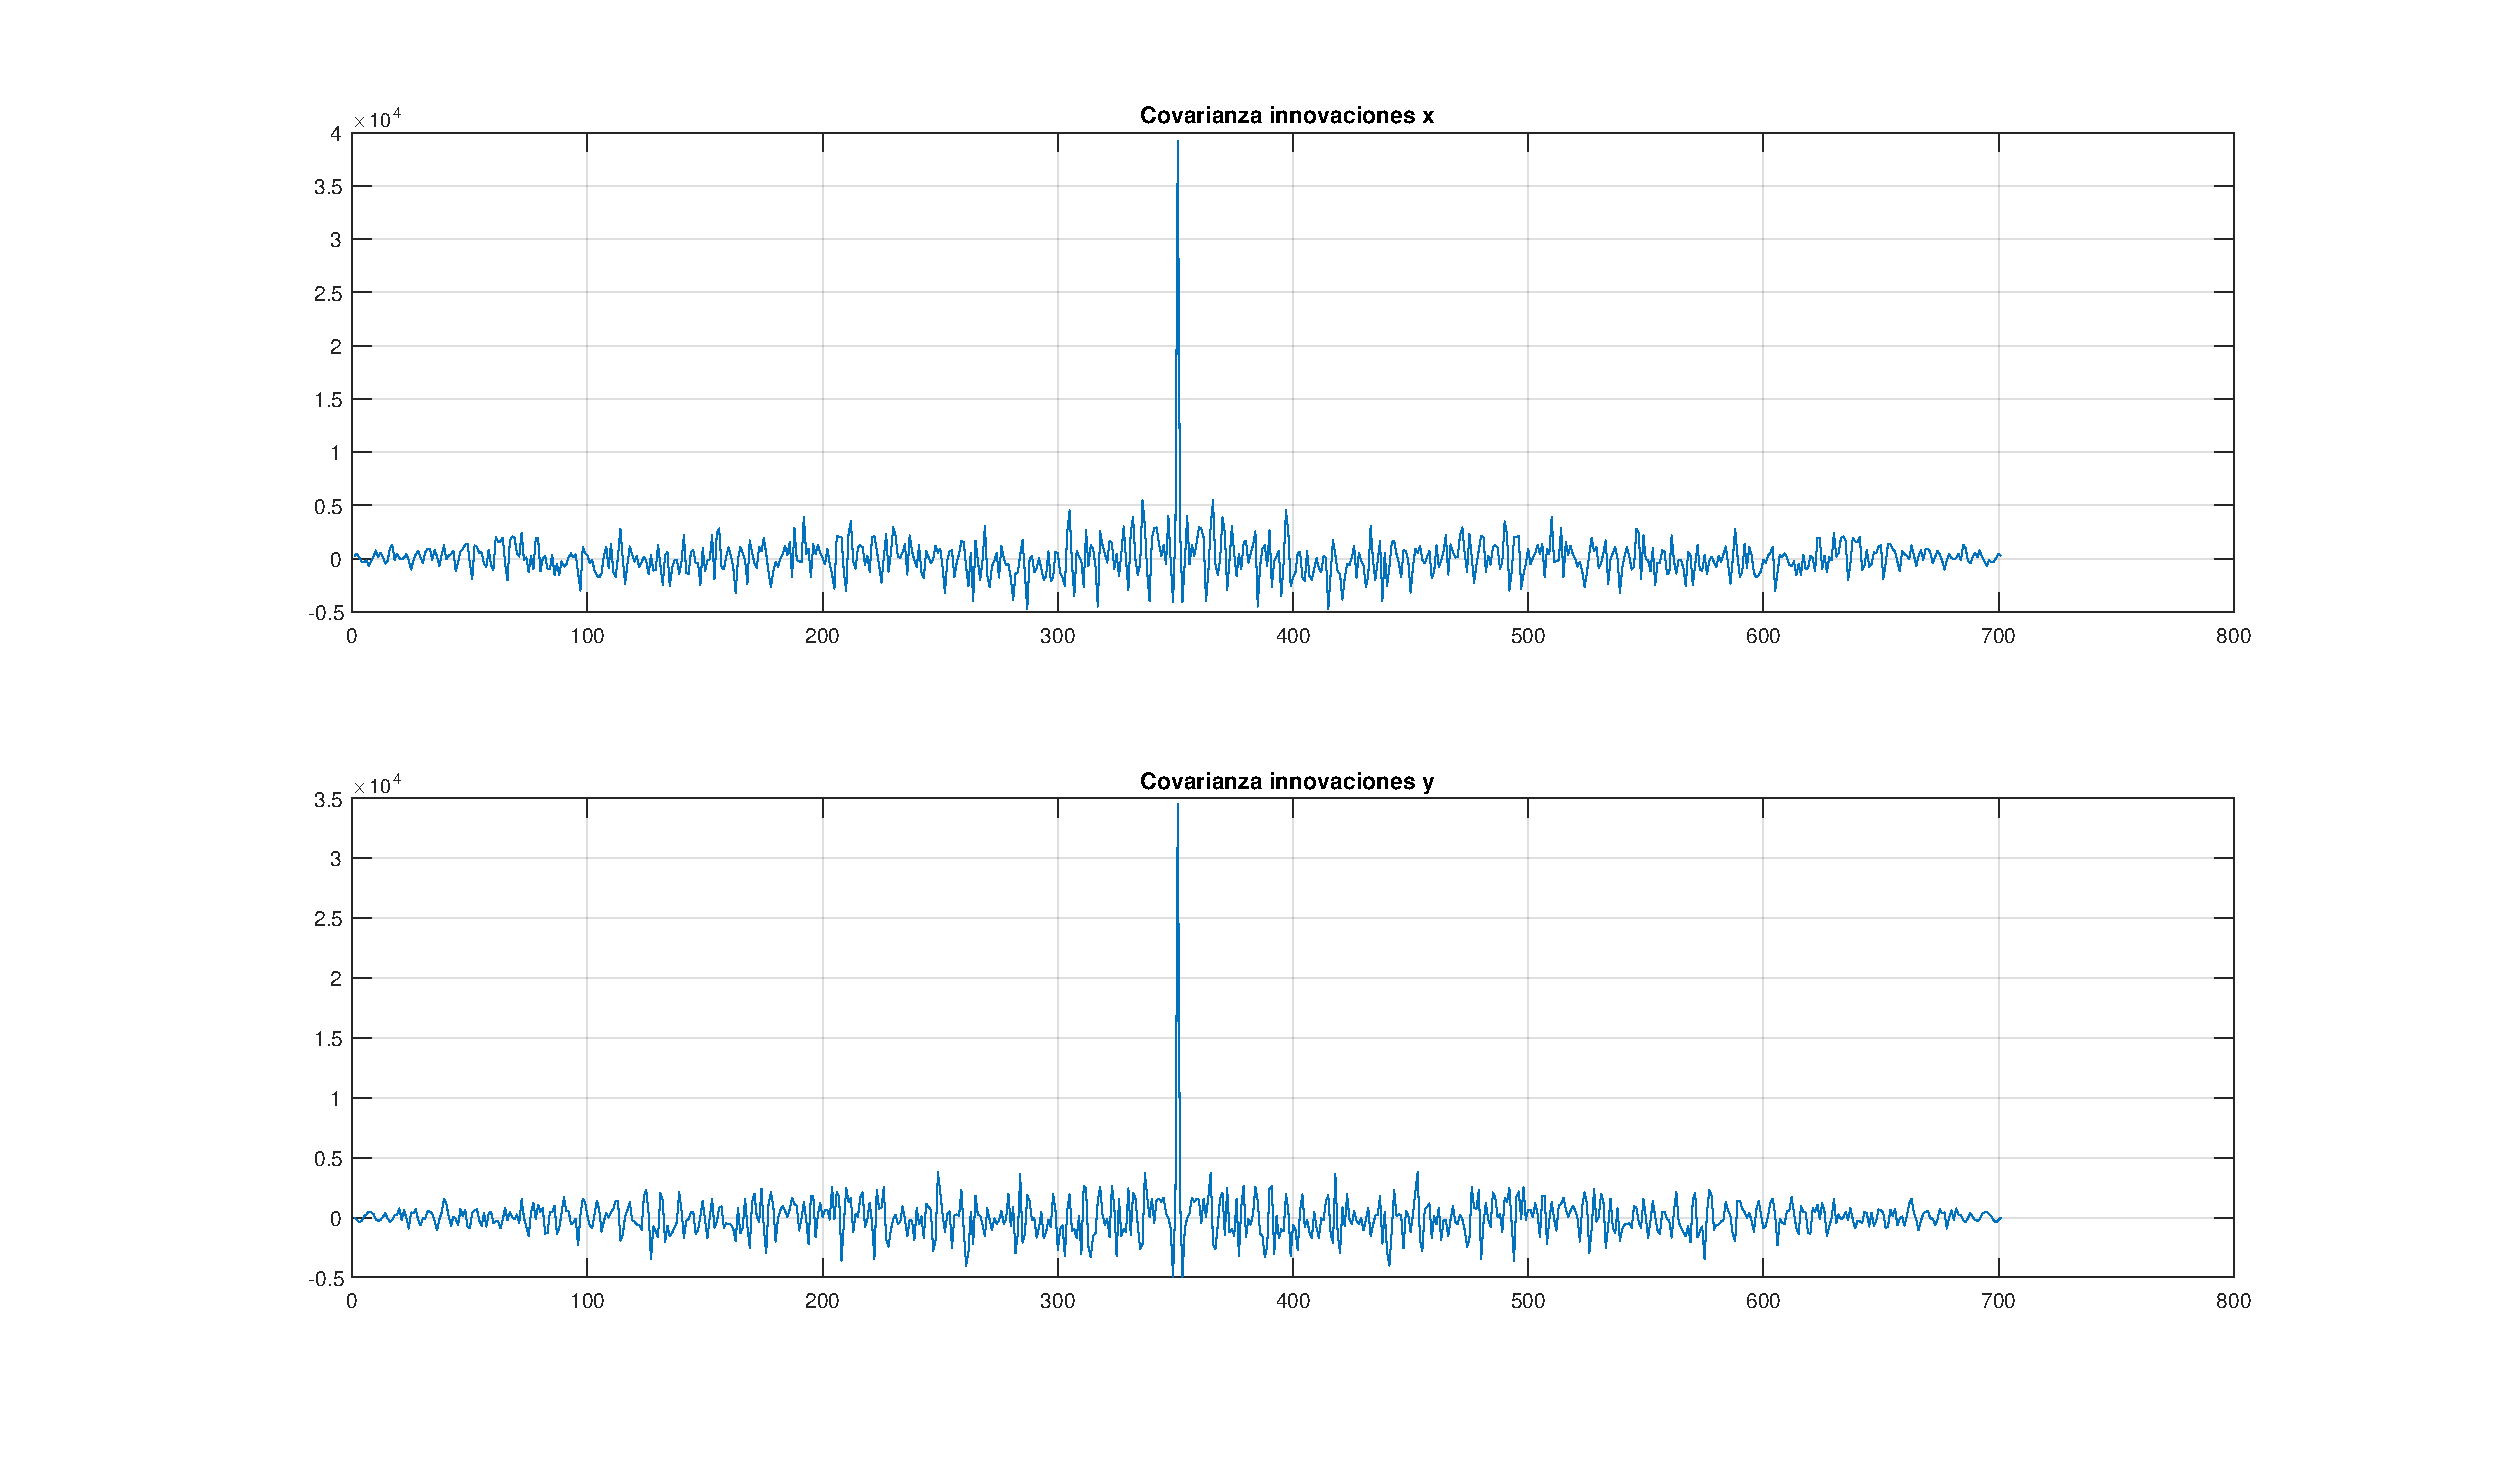
\includegraphics[width=1.0\textwidth,keepaspectratio]{Figuras/covinn_ej2b.pdf} \caption{Caso: Medición De Velocidad - Innovaciones} \label{fig:ej2b_innov}
		\end{figure}
			
		\subsubsection{Medición De Aceleración}
		
		En la figura \ref{fig:ej2c} observamos los resultados de la estimación basada en mediciones de aceleración. Puede verse que la trayectoria estimada nunca sigue a la real.
		
		\begin{figure}[H]
			\centering
			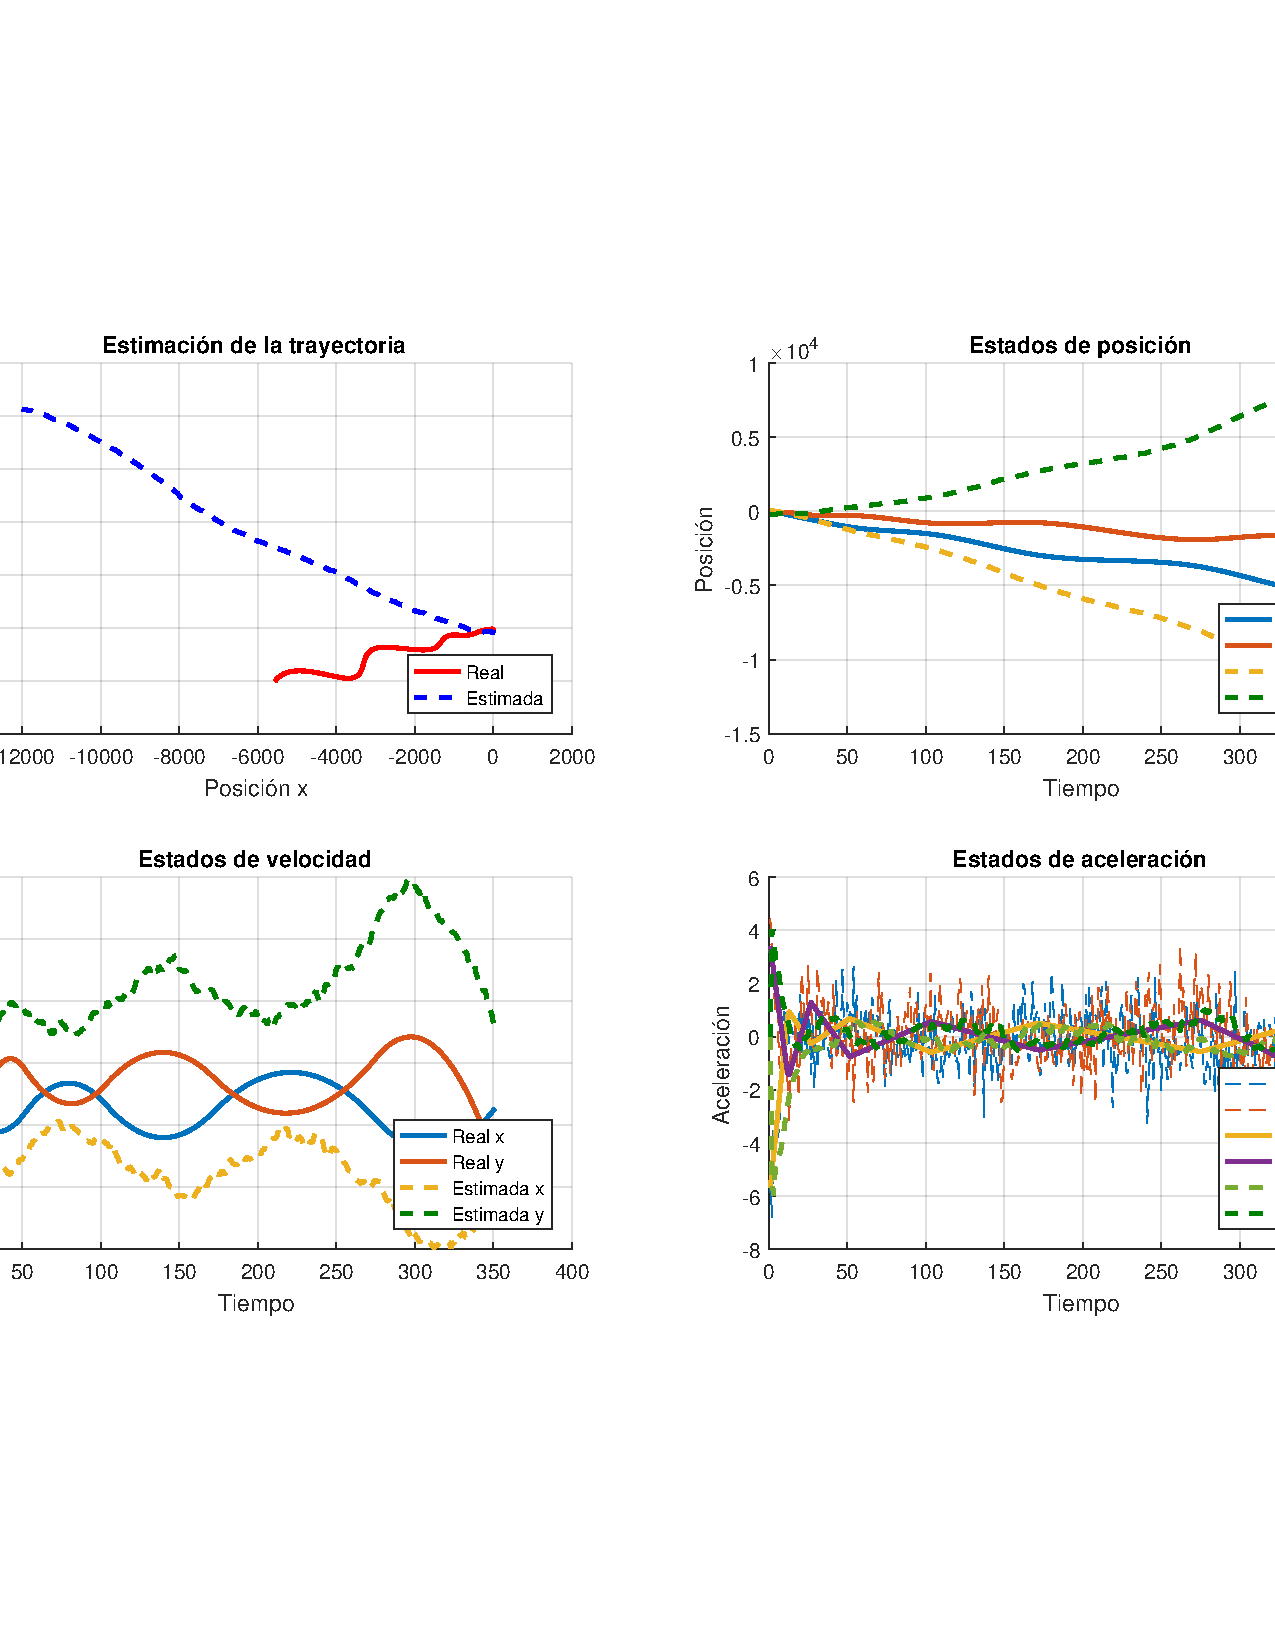
\includegraphics[scale=0.5,trim={6,5cm 0 0 0}]{Figuras/graf_ej2c.pdf}
			\caption{Caso: Medición De Aceleración}
			\label{fig:ej2c}
		\end{figure}
		
		En la figura \ref{fig:ej2c_innov} vemos la correlación de las innovaciones, donde se observa que se aproximan a un proceso blanco.
		
		\begin{figure}[H]
			\centering
			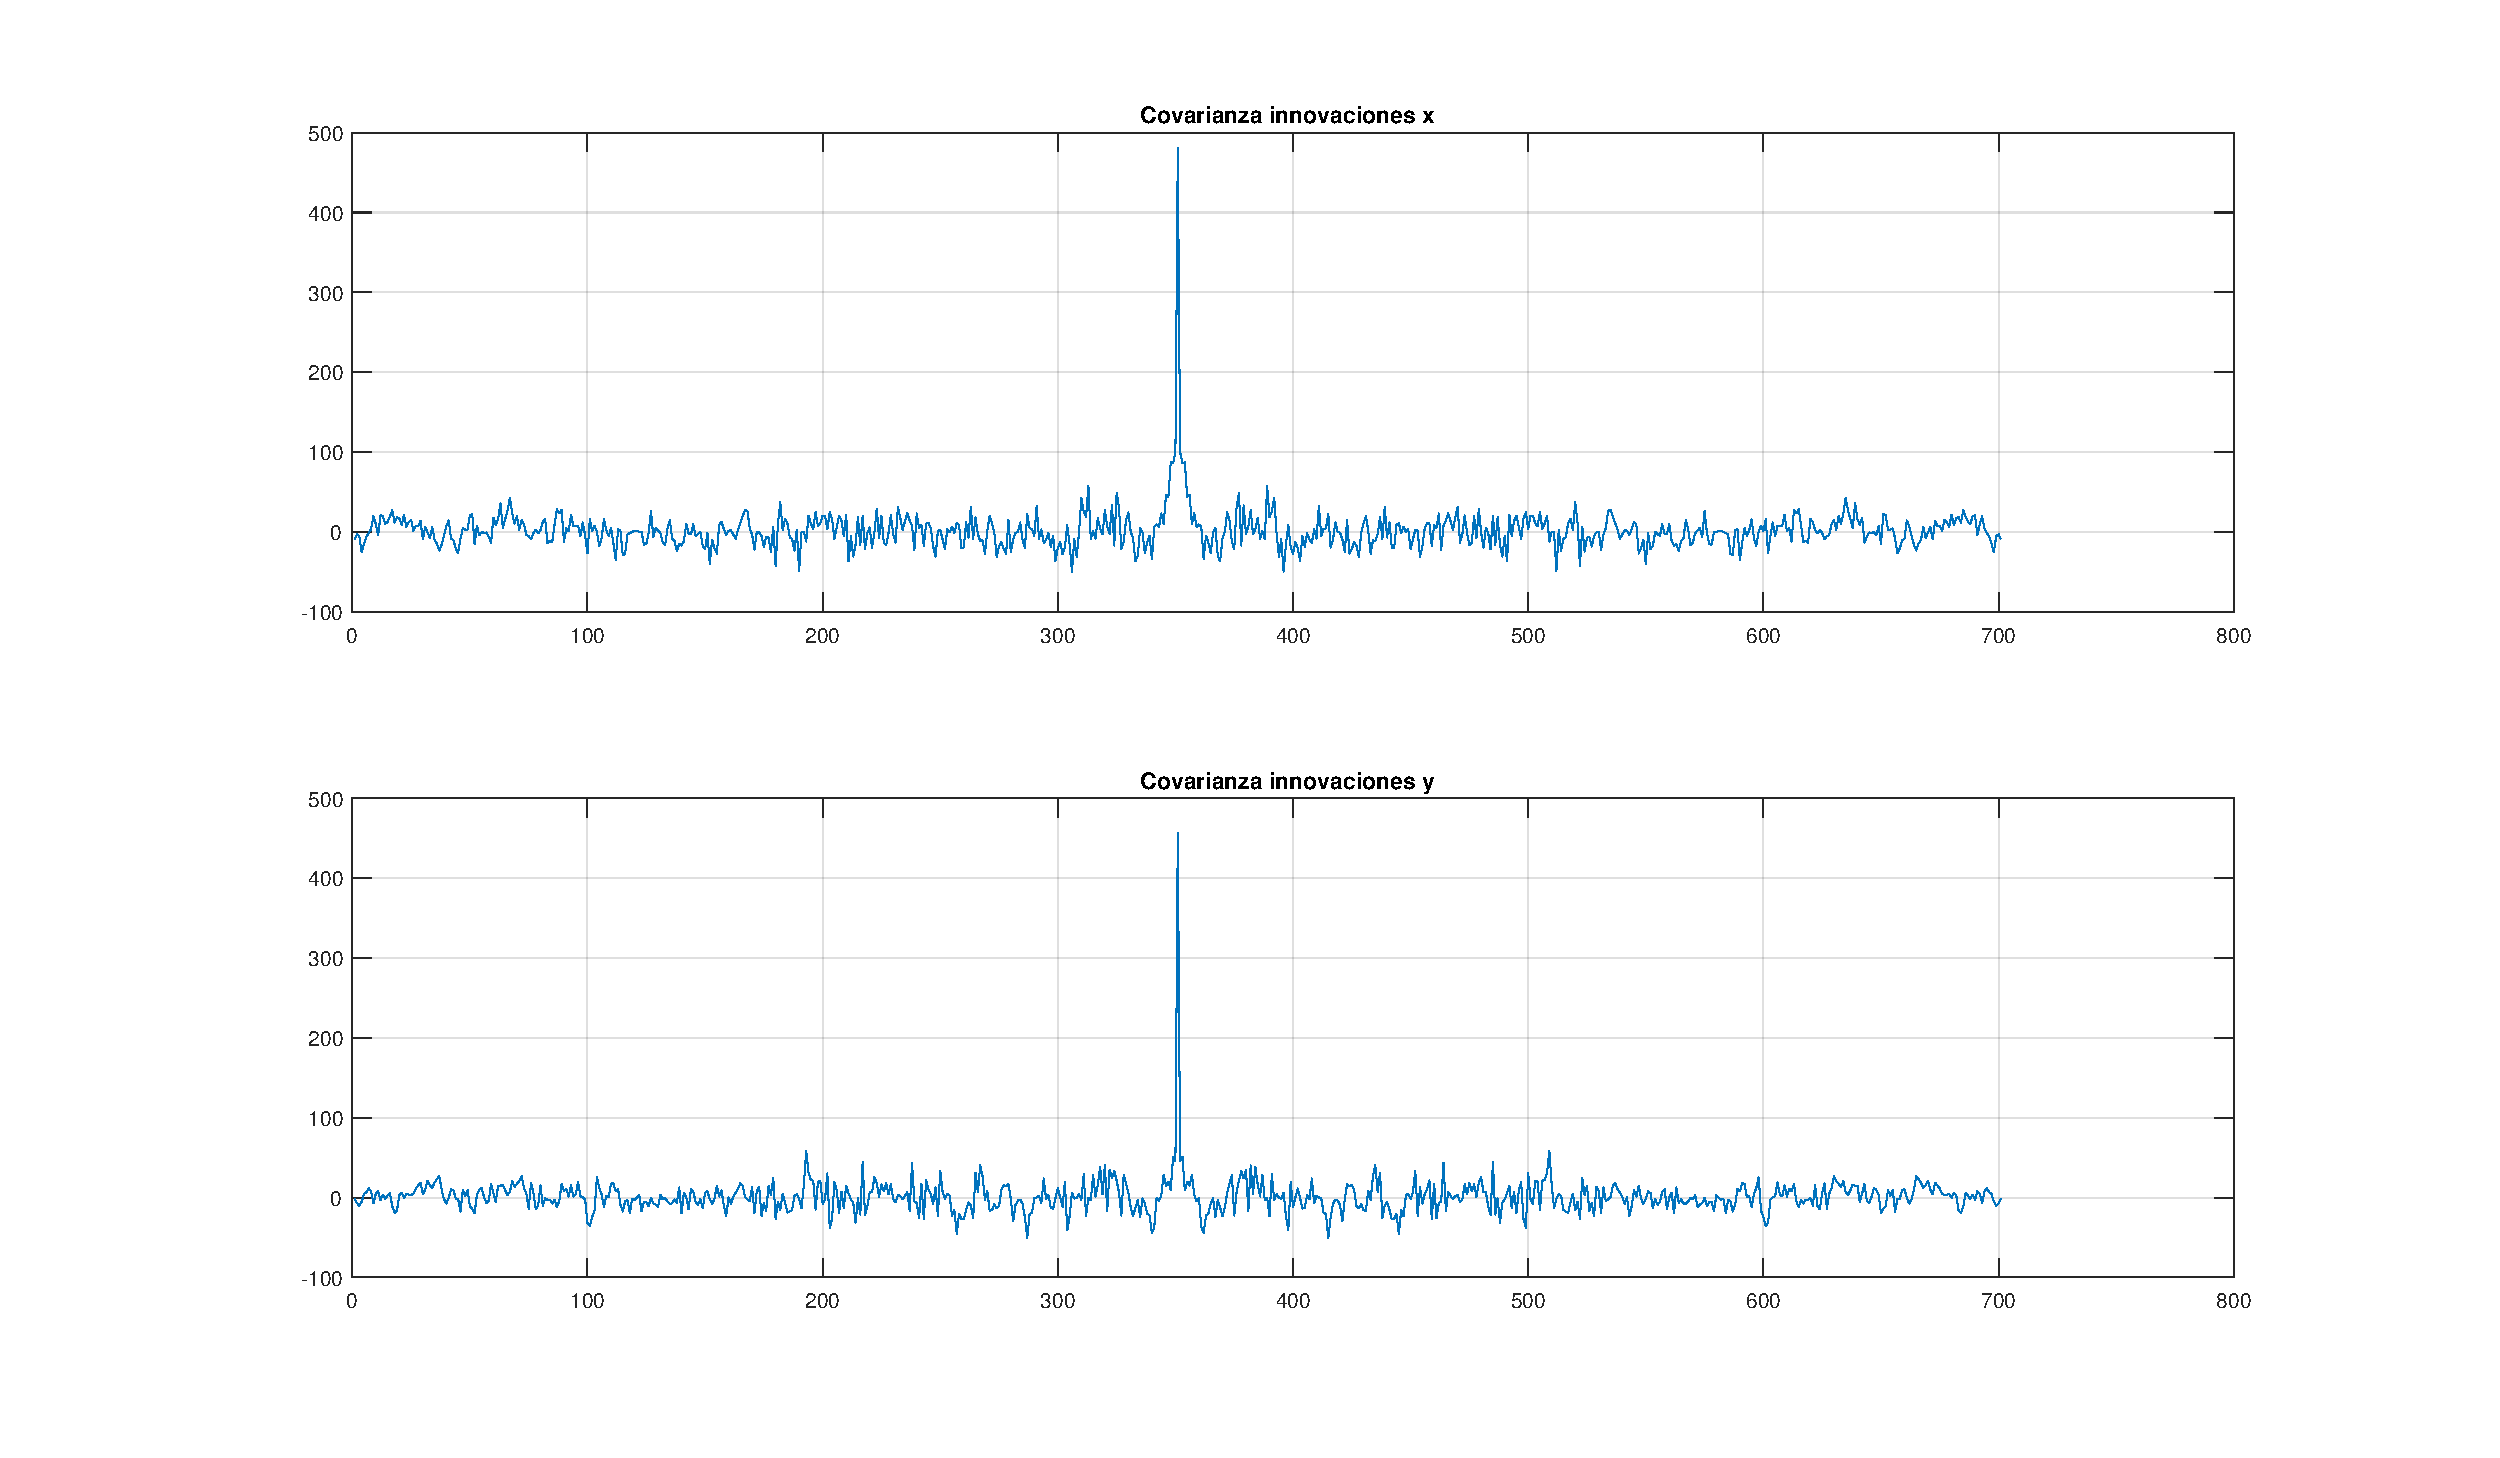
\includegraphics[width=1.0\textwidth,keepaspectratio]{Figuras/covinn_ej2c.pdf}
			\caption{Caso: Medición De Aceleración - Innovaciones}
			\label{fig:ej2c_innov}
		\end{figure}

	\subsection{Test De Observabilidad}
		Para determinar cuántos estados no observables tiene el sistema se debe analizar el rango de la \Juan{Si hay ganas y se acuerda alguno, podríamos explicar esto.. for extra points}
		matriz de observabilidad. A continuación se expone la porción de código que se encarga de ello:
		\lstinputlisting[firstline=243, firstnumber=243]{EJ2_full.m}

		Para los incisios del ejercicio \ref{sec:ej2} se obtiene la siguiente tabla.
		\begin{table}[h!]
			\centering
			\begin{tabular}{ccc}
				\toprule
				Medición	& Cantidad no observables	& Observables\\
				\midrule
				$\vect{p}$	& 0				& $\vect{p}$ $\vect{v}$ $\vect{a}$\\
				$\vect{v}$	& 2				& $\vect{p}$ $\vect{v}$ \\
				$\vect{a}$	& 4				& $\vect{p}$\\

				\bottomrule
			\end{tabular}
				\caption{Test de observabilidad para el ejercicio 2.}
				\label{tab:obs_ej2}
		\end{table}
%	\subsection{Script}
%	
%		A continuación presentamos el script de MATLAB que implementa el algoritmo. Se puede seleccionar si se esta midiendo posicion, velocidad o aceleracion, estableciendo las variables bool\_p, bool\_v o bool\_a en 1 o en 0 para indicar que se esta midiendo.
%	
%	%\lstinputlisting[]{../Octave/EJ2_full.m}
